\documentclass{report} % Utilisation de la classe 'report' pour prendre en charge les chapitres

% !TEX root = /Users/charleschikhani/Documents/L3/S6/Projet-MI/Rapport.tex

\usepackage[utf8]{inputenc}
\usepackage[T1]{fontenc}
\usepackage[french]{babel}
\usepackage{amsfonts}
\usepackage{amsmath}
\usepackage{amsthm}
\usepackage{amssymb}
\usepackage{graphicx}
\usepackage{hyperref}
\usepackage{eso-pic}
\usepackage{fancyhdr}
\usepackage{geometry}
\usepackage{tocloft}
\usepackage{titlesec}


% Définition des marges
\geometry{
  left=2.5cm,
  right=2.5cm,
  top=2.5cm,
  bottom=1.75cm,
}

% Définition du style de page "mypagestyle"
\fancypagestyle{mypagestyle}{
  \fancyhf{} % Efface tous les en-têtes et pieds de page existants
  \fancyhead[R]{
\includegraphics[width=3cm]{Ressources/Universite_Paris-Cite-logo.jpeg}} % En-tête droit avec l'image
  \fancyfoot[C]{\thepage} % Pied de page centré avec le numéro de page
  \renewcommand{\headrulewidth}{0.4pt} % Épaisseur de la ligne de séparation d'en-tête
  \renewcommand{\footrulewidth}{0pt} % Épaisseur de la ligne de séparation de pied de page
}

% Appliquer le style de page personnalisé
\pagestyle{mypagestyle}

% Ajustement de la taille de l'en-tête et de la police
\setlength{\headheight}{29.55806pt} % Hauteur de l'en-tête
\addtolength{\topmargin}{-17.55806pt} % Ajustement de la marge supérieure

\title{Qui a écrit Molière ?}
\author{CHIKHANI Charles \and ZAPFACK MESSIAN Jasen Steve \\ \and Encadrant : M. Hervé Fournier\\ \\ Université Paris Cité}
\date{02 Juin 2023}


\renewcommand{\thesection}{\arabic{section}}


\begin{document}
\maketitle
\tableofcontents

\newpage

\section{Introduction}

\vspace{\baselineskip}
\subsection{Présentation du sujet : la remise en question de l'attribution des pièces de Molière à l'auteur lui-même}
\vspace{\baselineskip}
\hspace{0,5cm}Depuis plusieurs décennies, une question persiste dans le domaine de la
littérature : l'attribution des pièces de Molière à l'auteur lui-même est-elle
remise en question ? Cette controverse a été initiée par Pierre Louÿs, un
romancier du XXe siècle, qui a suggéré que Pierre Corneille aurait pu être
l'auteur véritable des pièces de Molière. Cependant, cette théorie repose sur
des fondements fragiles et ne bénéficie d'aucune preuve concrète. Malgré cela,
la rumeur persiste, alimentée par des éléments tels que l'éclosion tardive de
Molière en tant qu'auteur, son prétendu manque d'éducation et de culture, ainsi
que l'absence de preuves manuscrites permettant de réfuter directement cette
hypothèse.
\subsection{Importance de l'analyse textuelle et statistique dans la résolution de cette question}
\vspace{\baselineskip}
\hspace{0,5cm}Au début des années 2000, Cyril et Dominique Labbé, deux chercheurs, ont avancé
l'idée selon laquelle Corneille aurait écrit pour Molière. Leur méthode consiste
à mesurer une "distance inter-textuelle" qui évalue la différence de lexique
entre les textes des deux auteurs. Si cette distance ne dépasse pas un certain
seuil, les deux pièces sont considérées comme écrites par le même auteur. Ils se
basent également sur le fait que de nombreux dramaturges de l'époque signaient
leurs œuvres sous le nom de "comédien poète", ce qui permettait aux véritables
auteurs de rester anonymes tout en bénéficiant de la promotion et de la
représentation de leurs pièces par les acteurs.


\hspace{0,5cm}Cependant, cette méthodologie a été contestée par d'autres chercheurs. Certains
ont souligné que l'implémentation de la méthode de Cyril et Dominique Labbé
pourrait "lisser artificiellement les différences entre les auteurs", en
utilisant une distance euclidienne qui accorde trop de poids aux lemmes
fréquents, réduisant ainsi la disparité entre les fréquences observées de
différentes formes. 
\\D'autres approches ont été proposées pour résoudre le problème de l'attribution
des comédies de Molière. Certaines méthodes utilisent une analyse textuelle et
statistique pour comparer les styles d'écriture, tandis que d'autres adoptent
des approches plus qualitatives en examinant les intrigues, la versification et
les sujets choisis dans les pièces.

\subsection{Hypothèses et problématique}
\vspace{\baselineskip}
\hspace{0,5cm} Dans ce rapport, nous examinerons deux hypothèses qui remettent
en question la
paternité des œuvres de Molière. La première hypothèse suggère que Molière
aurait fourni des brouillons à Pierre Corneille, qui aurait ensuite versifié les
pièces, peut-être avec l'aide de son frère. Selon cette hypothèse, Molière
aurait créé les intrigues, mais la versification aurait été réalisée par Pierre
Corneille, sans recevoir un crédit explicite. La deuxième hypothèse soutient que
Molière n'aurait ni écrit les intrigues ni les vers de ses pièces, et qu'il
n'aurait été qu'un nom célèbre utilisé pour promouvoir les pièces et dissimuler
le véritable auteur.

\hspace{0,5 cm} Pour résoudre cette controverse, différentes méthodes ont été
utilisées, chacune
avec ses propres avantages et limitations. L'objectif de cette étude est
d'évaluer ces approches et de fournir une analyse critique des résultats
obtenus.
\\Pour ce faire, dans la section suivante, nous présenterons en détail l'article de Florian
Cafiero et Jean-Baptiste Camps, qui examine cette question en utilisant une
analyse textuelle et statistique. Nous aborderons les différentes perspectives
et critiques soulevées par d'autres chercheurs, ainsi que les différentes
approches méthodologiques qui ont été utilisées pour résoudre le problème de
l'attribution des pièces de Molière.


Le rapport qui suit explorera en profondeur ces différentes approches et tentera
de faire la lumière sur cette controverse persistante, fournissant ainsi une
contribution significative à notre compréhension de l'œuvre de Molière et de son
véritable auteur.


\section{Compréhension de l'article de Florian Cafiero et Jean-Baptiste Camps}

\subsection{Contexte et objectifs de l'étude}
\subsection{Méthodologie utilisée}
\subsection{Formalisation du problème de l'attribution des pièces de théâtre}
\subsection{Approche adoptée pour résoudre le problème}
\subsection{Présentation et analyse des résultats obtenus}

\section{Notre expérience}

\vspace{\baselineskip}
\subsection{Description de l'expérience que nous avons menée}
\vspace{\baselineskip}
\hspace{0,5cm}Dans le cadre de cette étude, nous avons mené une expérience visant à déterminer
la paternité des textes de Molière. L'objectif principal était de développer une
méthodologie pour identifier les caractéristiques distinctives du style
d'écriture de Molière et les comparer à ceux d'autres auteurs de la même époque.
Le second objectif était de mieux comprendre les enjeux du choix des
caractéristiques.
Pour cela, nous avons utilisé des techniques d'analyse textuelle et statistique
pour extraire des informations à partir des textes et les utiliser comme base
pour la classification. 
\subsection{Choix des outils d'analyse textuelle et statistique utilisés}
\vspace{\baselineskip}
\hspace{0,5cm}Pour mener notre analyse, nous avons choisi plusieurs outils d'analyse textuelle
et statistique. Nous avons opté pour la bibliothèque \textbf{NLTK} (\textit{Natural Language
Toolkit}) de Python pour ses fonctionnalités de prétraitement de texte, telles
que la suppression des \textit(stopwords), la normalisation des mots et la lemmatisation.
Cette bibliothèque nous a permis de nettoyer les données textuelles et de
réduire les informations redondantes ou inutiles.
\\En ce qui concerne l'analyse statistique, nous avons utilisé des techniques
telles que l'analyse de fréquence des mots, l'analyse des \textit{n-grammes} et l'analyse
de similarité. Pour ces tâches, nous avons utilisé des bibliothèques \textit{Python}
telles que \textit{scikit-learn}, qui offre des fonctionnalités avancées pour l'analyse
de texte et la classification.

\subsection{Méthodologie mise en place}
\vspace{\baselineskip}
\hspace{0,5cm}La méthodologie mise en œuvre repose sur un ensemble d'étapes
soigneusement orchestrées : \\La collecte des données a été réalisée avec
rigueur et minutie. Une vaste compilation d'œuvres signées Molière ainsi que
celles d'autres auteurs contemporains a été rassemblée afin de constituer le
corpus de textes sur lequel s'appuie notre étude.  \\Le prétraitement des
données a été effectué avec une approche méthodologique précise. Des techniques
de prétraitement textuel sophistiquées ont été appliquées pour purifier les
données, éliminant ainsi les éléments superflus et les interférences
indésirables. Parmi ces techniques, on compte la suppression des stopwords, la
normalisation des mots et la lemmatisation.  \\L'analyse des caractéristiques
textuelles a été entreprise avec une attention particulière portée à chaque
auteur. Par le biais de techniques d'analyse textuelle avancées, notamment
l'analyse de fréquence des mots, l'exploration des n-grammes et l'évaluation de
la similarité, nous avons extrait et étudié en profondeur les traits
caractéristiques propres au style d'écriture de chacun.  \\La classification des
textes a constitué une étape cruciale de notre démarche.  Nous avons employé des
méthodes de classification établies, telles que les arbres de décision et les
algorithmes de classification bayésienne, pour attribuer à chaque segment de
texte son auteur d'origine, qu'il s'agisse de Molière ou d'un autre écrivain de
référence. 

\hspace{0,5cm}Notre expérience s'est divisée en deux axes. Le premier axe
consiste à déterminer comprendre et étudier le style d'écriture de Molière. Le
second axe consiste à déterminer les clusters de textes qui se ressemblent le
plus.

\hspace{0,5cm}Grâce à la bibliothèque \textbf{NLTK} et \textbf{WorldCloud}, nous
avons pu faire un nuage de mot pour le corpus de Molière. Un nuage de mots est
une manière de visualiser la fréquence des mots dans un corpus. Les mots
les plus fréquents sont présentés sous forme de nuage, où la taille du mot est
proportionnelle à sa fréquence. Cette représentation peut donner une vue
d'ensemble rapide des termes les plus courants dans le corpus de Molière. Pour
que l'analyse soit plus pertinente nous avons supprimé la prise en compte des
noms propres, qui sont uniques aux oeuvres.

\begin{figure}[htbp]
    \centering
    \includegraphics[width=15cm]{Ressources/nuage_sans_noms.png}
    \caption{Nuage de mots du corpus de Molière}
    \label{fig:images}
  \end{figure}

\vspace{\baselineskip}

\hspace{0,5cm}Grâce au nuage de mots, nous avions remarqué que le mot \textit{Monsieur}
revenait très souvent. Cette grande importance du mot \textit{Monsieur} dans le
nuage de mots révèle le vocabulaire et les règles d'écriture de l'époque.
\\Afin de mieux comprendre le style d'écriture de Molière, nous avons également
réaliser un histograme des mots les plus fréquents dans le corpus de Molière.
Pour rendre ce diagramme plus pertinent, nous avons décidé de ne pas prendre en
compte les noms de personnages mais également le mot \textit{Monsieur}.

\begin{figure}[htbp]
    \centering
    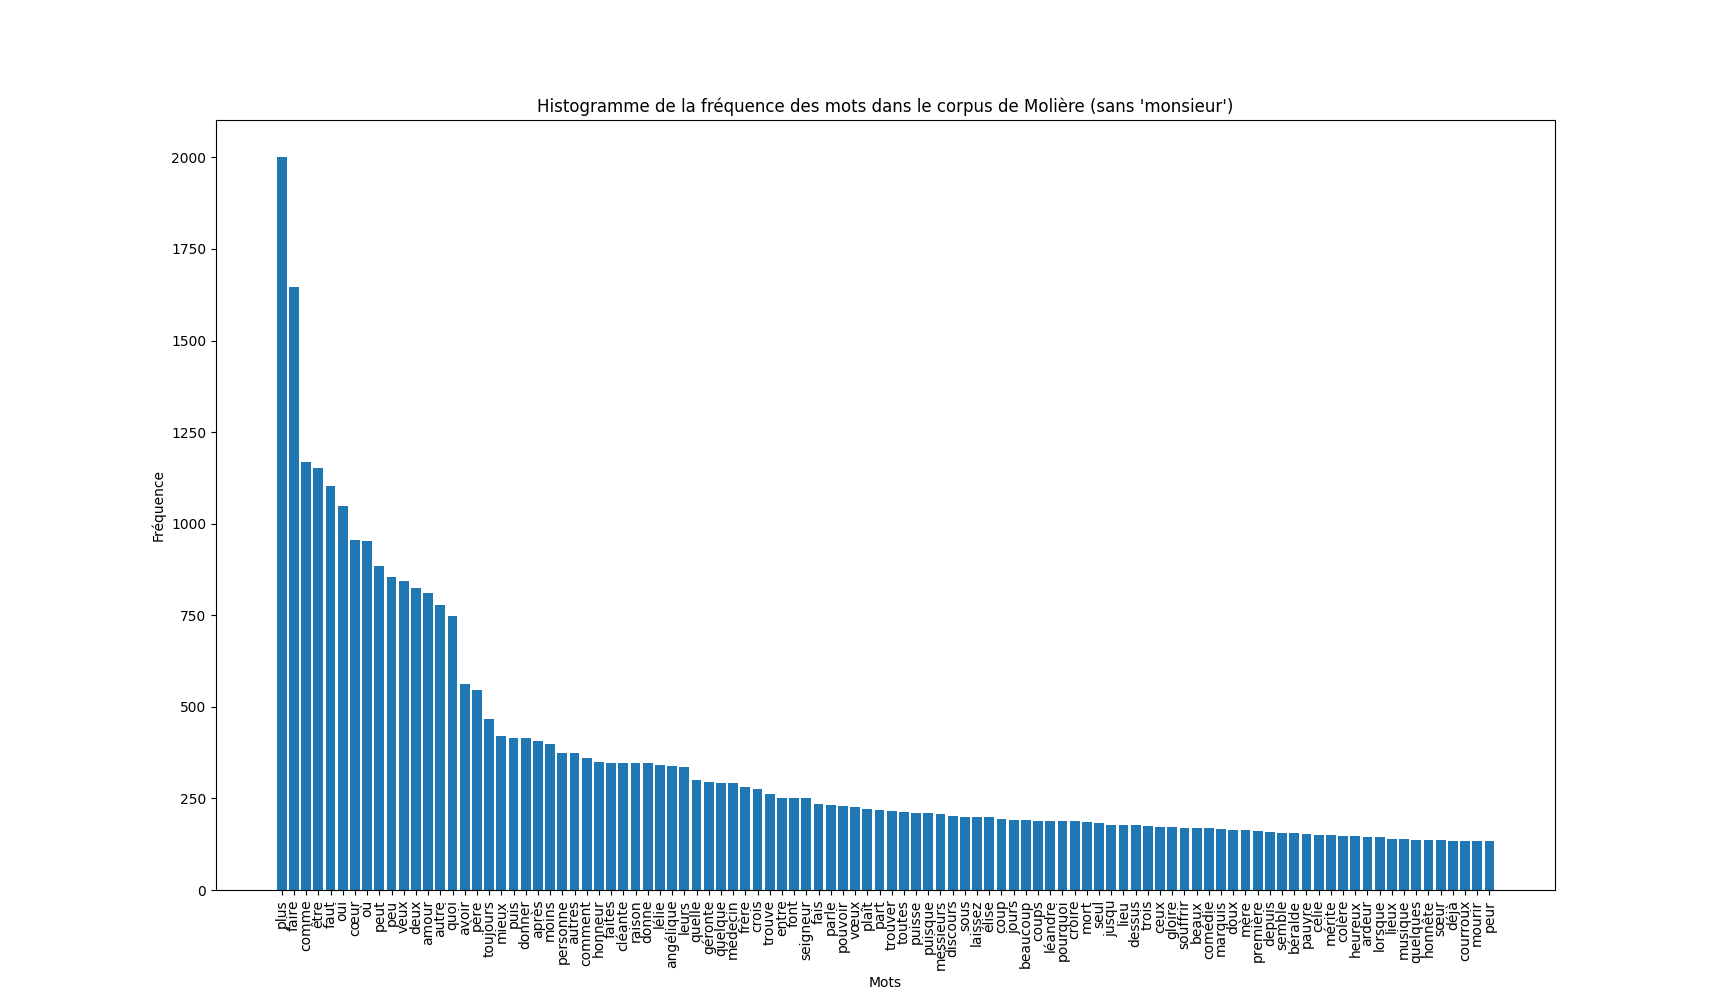
\includegraphics[width=13cm]{Ressources/diagr_sans_noms_mosn.png}
    \caption{Diagramme de mots du corpus de Molière sans le mot \textit{Monsieur}}
    \label{fig:images}
  \end{figure}

  \vspace{\baselineskip}


\subsection{Collecte et préparation des données}
\vspace{\baselineskip}
Pour notre expérience, nous avons collecté une collection d'œuvres de Molière,
ainsi que des œuvres d'autres auteurs de la même époque. Ces données ont été
recueillies à partir de sources disponibles en ligne et ont été soigneusement
sélectionnées pour représenter différents genres et styles d'écriture.

Avant de procéder à l'analyse, nous avons effectué un prétraitement des données.
Cela comprenait la suppression des stopwords (mots courants sans grande
signification), la normalisation des mots (mise en minuscules) et la
lemmatisation (réduction des mots à leur forme canonique). Ce processus de
prétraitement nous a permis de nettoyer les données et d'éliminer les éléments
perturbateurs qui pourraient fausser nos résultats.

\subsection{Analyse des résultats obtenus et comparaison avec l'article de référence}
\vspace{\baselineskip}

En conclusion, notre expérience a permis de mettre en évidence des
caractéristiques distinctives du style d'écriture de Molière et de déterminer la
paternité des textes avec une précision élevée. Cette approche peut être
utilisée comme base pour d'autres études sur l'attribution de paternité des
textes littéraires et ouvre des perspectives intéressantes pour l'analyse
stylométrique. 

\section{Perspectives et réflexions}

\subsection{Approfondissement des techniques de linguistique quantitative pour déterminer la paternité d'un texte}
\subsection{Réflexion sur les aspects algorithmiques impliqués dans l'analyse textuelle et statistique}
\subsection{Limitations de notre expérience et suggestions pour de futures recherches}

\section{Conclusion}

\subsection{Récapitulation des principales conclusions de l'article de Florian Cafiero et Jean-Baptiste Camps}
\subsection{Résumé des résultats de notre expérience et leur concordance ou divergence avec l'article}
\subsection{Implications de cette étude dans le domaine de l'attribution des œuvres littéraires}

\end{document}
